%% start of file `template.tex'.
%% Copyright 2006-2015 Xavier Danaux (xdanaux@gmail.com).
%
% This work may be distributed and/or modified under the
% conditions of the LaTeX Project Public License version 1.3c,
% available at http://www.latex-project.org/lppl/.


\documentclass[11pt,a4paper,sans]{moderncv}        % possible options include font size ('10pt', '11pt' and '12pt'), paper size ('a4paper', 'letterpaper', 'a5paper', 'legalpaper', 'executivepaper' and 'landscape') and font family ('sans' and 'roman')
\usepackage{ragged2e}
\usepackage{lastpage}
%\usepackage[german]{babel} 
\usepackage{fancyhdr}

%\fancyfoot[C]{ \thepage\ / \pageref{LastPage}}
\usepackage{pdfpages}
% moderncv themes
\moderncvstyle{classic}
\usepackage{xpatch}
\xpatchcmd{\makeletterclosing}{[3em]}{[2em]}{}{}%abstand nach closing                           % style options are 'casual' (default), 'classic', 'banking', 'oldstyle' and 'fancy'
\moderncvcolor{blue}                               % color options 'black', 'blue' (default), 'burgundy', 'green', 'grey', 'orange', 'purple' and 'red'
%\renewcommand{\familydefault}{\sfdefault}         % to set the default font; use '\sfdefault' for the default sans serif font, '\rmdefault' for the default roman one, or any tex font name
%\nopagenumbers{}                                  % uncomment to suppress automatic page numbering for CVs longer than one page

% character encoding
%\usepackage[utf8]{inputenc}                       % if you are not using xelatex ou lualatex, replace by the encoding you are using
%\usepackage{CJKutf8}                              % if you need to use CJK to typeset your resume in Chinese, Japanese or Korean
\renewcommand*{\namefont}{\fontsize{20}{40}\mdseries\upshape}

% adjust the page margins
\usepackage[scale=0.75]{geometry}
%\setlength{\hintscolumnwidth}{3cm}                % if you want to change the width of the column with the dates
%\setlength{\makecvtitlenamewidth}{10cm}           % for the 'classic' style, if you want to force the width allocated to your name and avoid line breaks. be careful though, the length is normally calculated to avoid any overlap with your personal info; use this at your own typographical risks...



% personal data
\name{Fabian }{Gruber}
%\title{Resumé title}                               % optional, remove / comment the line if not wanted
\address{Anna-Stainer-Knittel-Weg 3/5/4}{6020 Innsbruck}% optional, remove / comment the line if not wanted; the "postcode city" and "country" arguments can be omitted or provided empty
\phone[mobile]{+43~650~2587521}                   % optional, remove / comment the line if not wanted; the optional "type" of the phone can be "mobile" (default), "fixed" or "fax"
%\phone[fixed]{+2~(345)~678~901}
%\phone[fax]{+3~(456)~789~012}
\email{Fabian.Gruber@uibk.ac.at}                               % optional, remove / comment the line if not wanted
%\homepage{www.johndoe.com}                         % optional, remove / comment the line if not wanted
%\social[linkedin]{john.doe}                        % optional, remove / comment the line if not wanted
%\social[twitter]{jdoe}                             % optional, remove / comment the line if not wanted
%\social[github]{jdoe}                              % optional, remove / comment the line if not wanted
%\extrainfo{additional information}                 % optional, remove / comment the line if not wanted
\photo[64pt][0.2pt]{Foto_FabianGruber}                       % optional, remove / comment the line if not wanted; '64pt' is the height the picture must be resized to, 0.4pt is the thickness of the frame around it (put it to 0pt for no frame) and 'picture' is the name of the picture file
%\quote{}                                 % optional, remove / comment the line if not wanted

% bibliography adjustements (only useful if you make citations in your resume, or print a list of publications using BibTeX)
%   to show numerical labels in the bibliography (default is to show no labels)
\makeatletter\renewcommand*{\bibliographyitemlabel}{\@biblabel{\arabic{enumiv}}}\makeatother
%   to redefine the bibliography heading string ("Publications")
%\renewcommand{\refname}{Articles}

% bibliography with mutiple entries
\usepackage{multibib}
%\newcites{book,misc}{{Books},{Others}}
%----------------------------------------------------------------------------------
%            content
%----------------------------------------------------------------------------------
\begin{document}
\renewcommand*{\bibliographyhead}[1]{}
%\begin{CJK*}{UTF8}{gbsn}                          % to typeset your resume in Chinese using CJK

%-----       letter       ---------------------------------------------------------
% recipient data
\recipient{Mag. Christoph Stenitzer}{AGES - \"{O}sterreichische Agentur f\"ur Gesundheit und Ern\"ahrungssicherheit GmbH\\Spargelfeldstra{\ss}e 191\\1220 Wien}
\date{26. Februar 2018}
\opening{\textbf{Betreff: Bewerbung als Fachexperte/in f\"ur das Institut Pflanzenschutzmittel, Abteilung
Umweltverhalten} \\[0.5cm]     Sehr geehrter Herr Stenitzer!}
\closing{Mit besten Gr\"{u}{\ss}en,}
%\enclosure[Anhang]{Lebenslauf, Diplombescheid und Zeugnis der zweiten Diplompr\"ufung}       % use an optional argument to use a string other than "Enclosure", or redefine \enclname

\makelettertitle
\justify
\vspace{-0.5cm} % kleinerer Abstand

Nach mehreren Jahren der T\"atigkeit an Universit\"aten m\"ochte ich ein neues Kapitel aufschlagen und mich f\"ur die ausgeschriebene Stelle bewerben. An dieser reizt mich sowohl die M\"oglichkeit, weiterhin wissenschaftlich im Bereich Bodenkunde t\"atig zu sein, als auch die Herausforderung, einen Beitrag in einem so spannenden Themengebiet wie der Umweltwirkung von Pflanzenschutzmittel leisten zu k\"onnen.

Seit meinem Studium der Kulturtechnik und Wasserwirtschaft besch\"aftige ich mich mit Modellierung und Bodenkunde. Am Institut f\"ur Angewandte Geologie der BOKU Wien sammelte ich als Diplomand und sp\"ater Projektmitarbeiter erste Erfahrungen in der Anwendung von Simulationssoftware im Bereich Naturgefahren, etwa bei der Modellierung von Dammbr\"uchen (BREACH), hydraulischer und hydrologischer Modellierung (FLO-2D) oder Massenbewegungen (RAMMS, DAN3D). In Bezug auf die Wirkung von Schadstoffen absolvierte ich in dieser Zeit auch die Lehrveranstaltung \emph{Risk assessment in the aquatic environment}. W\"ahrend meiner T\"atigkeit in der Arbeitsgruppe \emph{Boden und Landschafts\"okologie} des Instituts f\"ur Geographie der Universit\"at Innsbruck hat sich mein Fokus auf die statistische Modellierung von Gel\"ande- und Bodenparametern mit geographischen Informationssystemen und der Programmiersprache R verschoben. Im Rahmen meiner Besch\"aftigung mit Bodenfunktionsevaluierung untersuchte ich den Einfluss von Topographie f\"ur die Regionalisierung der  einzelnen Bodenfunktionen wie Transformations- oder R\"uckhaltepotenzial und absolvierte Lehrveranstaltungen zum Thema Bodenmikrobiologie.

Meine langj\"ahrige Erfahrung in der Anwendung und Validierung verschiedenster Modellierungsans\"atze erleichtert mir den Einsatz von Simulationsprogrammen und die Einsch\"atzung von Modellergebnissen und deren St\"arken und Schw\"achen. Neben einer allgemeinen Begeisterung f\"ur  Umweltthemen und Landwirtschaft bringe ich Erfahrung in der Analyse komplexer Daten, Freude an der Arbeit in interdisziplin\"aren Teams sowie  die Bereitschaft, mir notwendige Sachkenntnis rasch und selbstst\"andig anzueignen, mit.%[-0.7cm]
%\vspace{-0.1cm}

\"Uber eine Einladung zu einem Gespr\"ach w\"urde ich mich freuen.

\makeletterclosing
%\vspace{-1.5cm}
\clearpage


% Publications from a BibTeX file without multibib
%  for numerical labels: \renewcommand{\bibliographyitemlabel}{\@biblabel{\arabic{enumiv}}}% CONSIDER MERGING WITH PREAMBLE PART
%  to redefine the heading string ("Publications"): 
%\renewcommand{\refname}{Publikationen}
\nocite{*}
\bibliographystyle{plain}
\bibliography{publications3}   
%\clearpage\end{CJK*}                              % if you are typesetting your resume in Chinese using CJK; the \clearpage is required for fancyhdr to work correctly with CJK, though it kills the page numbering by making \lastpage undefined
%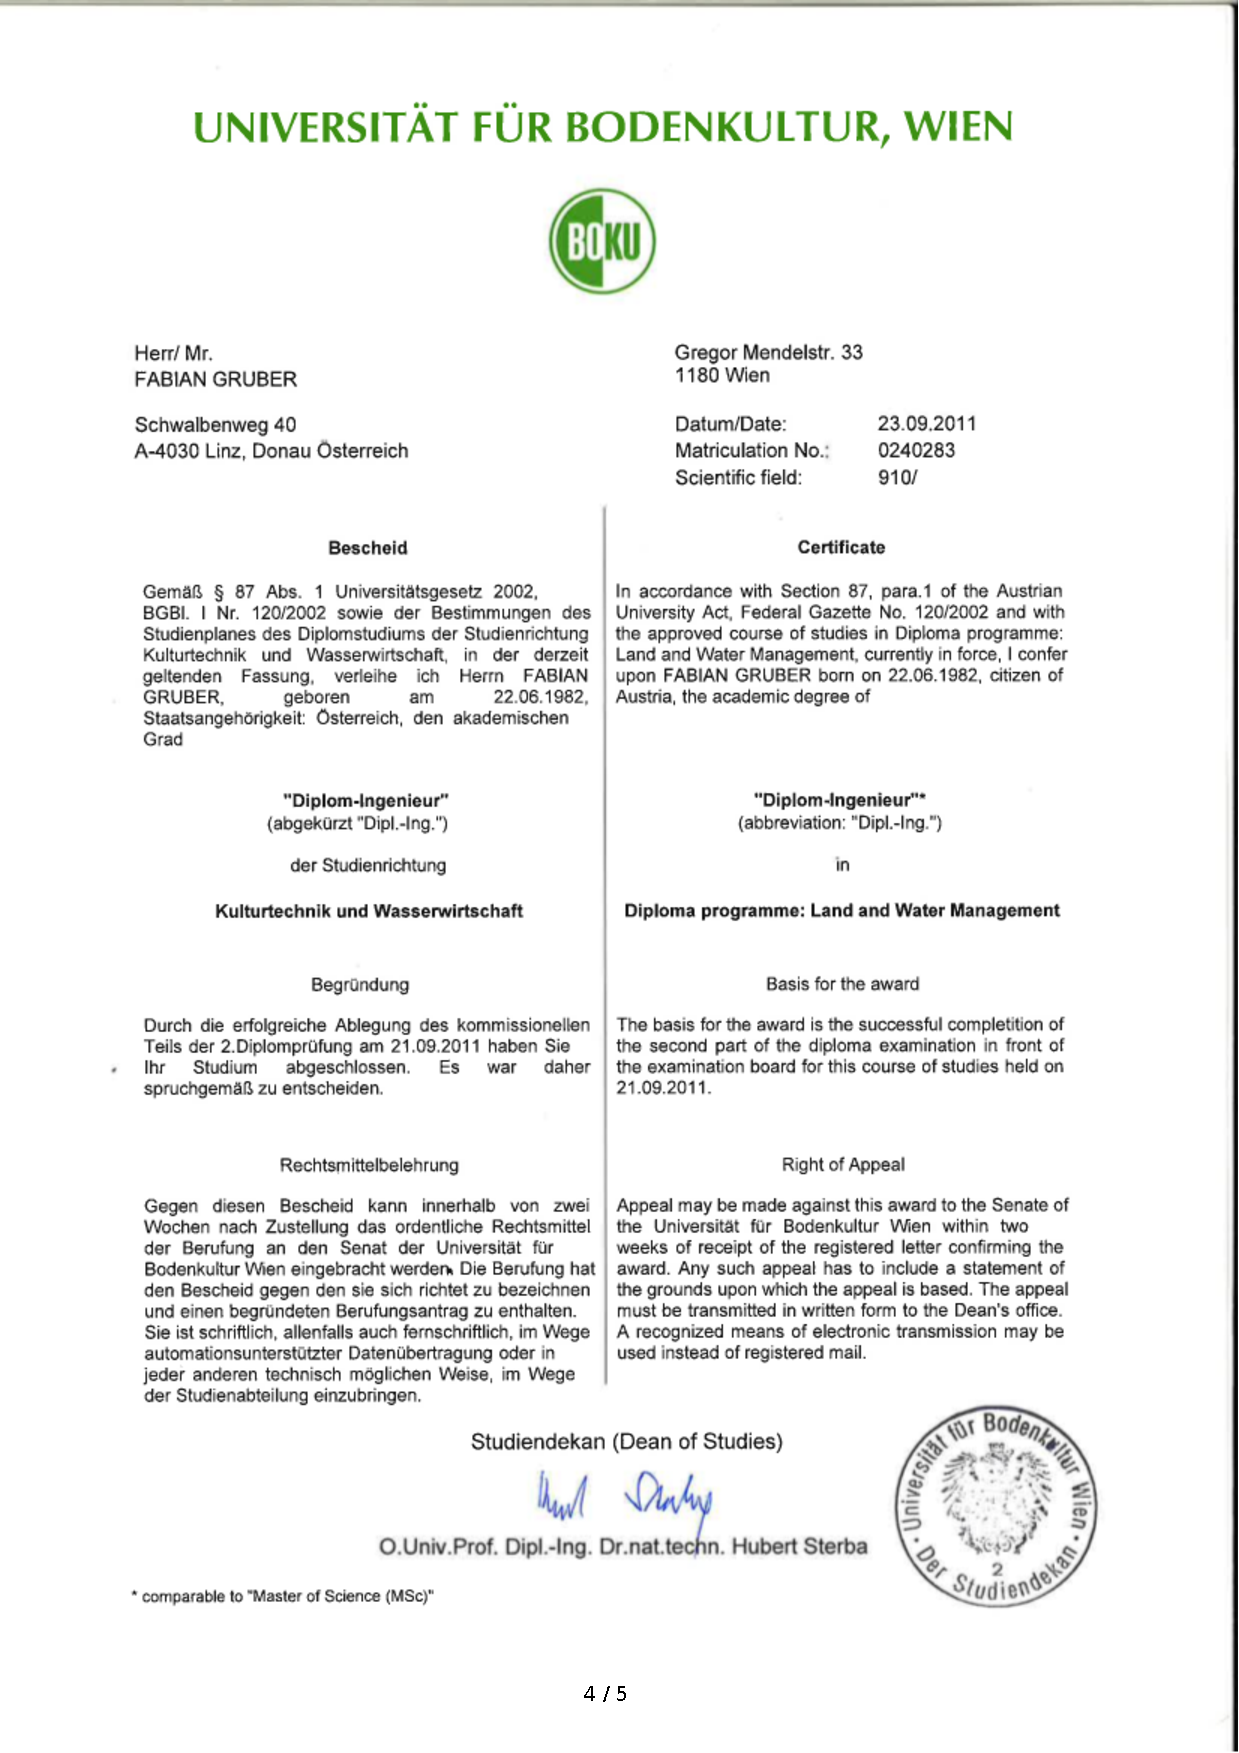
\includepdf{DP_seite4von5.pdf}
%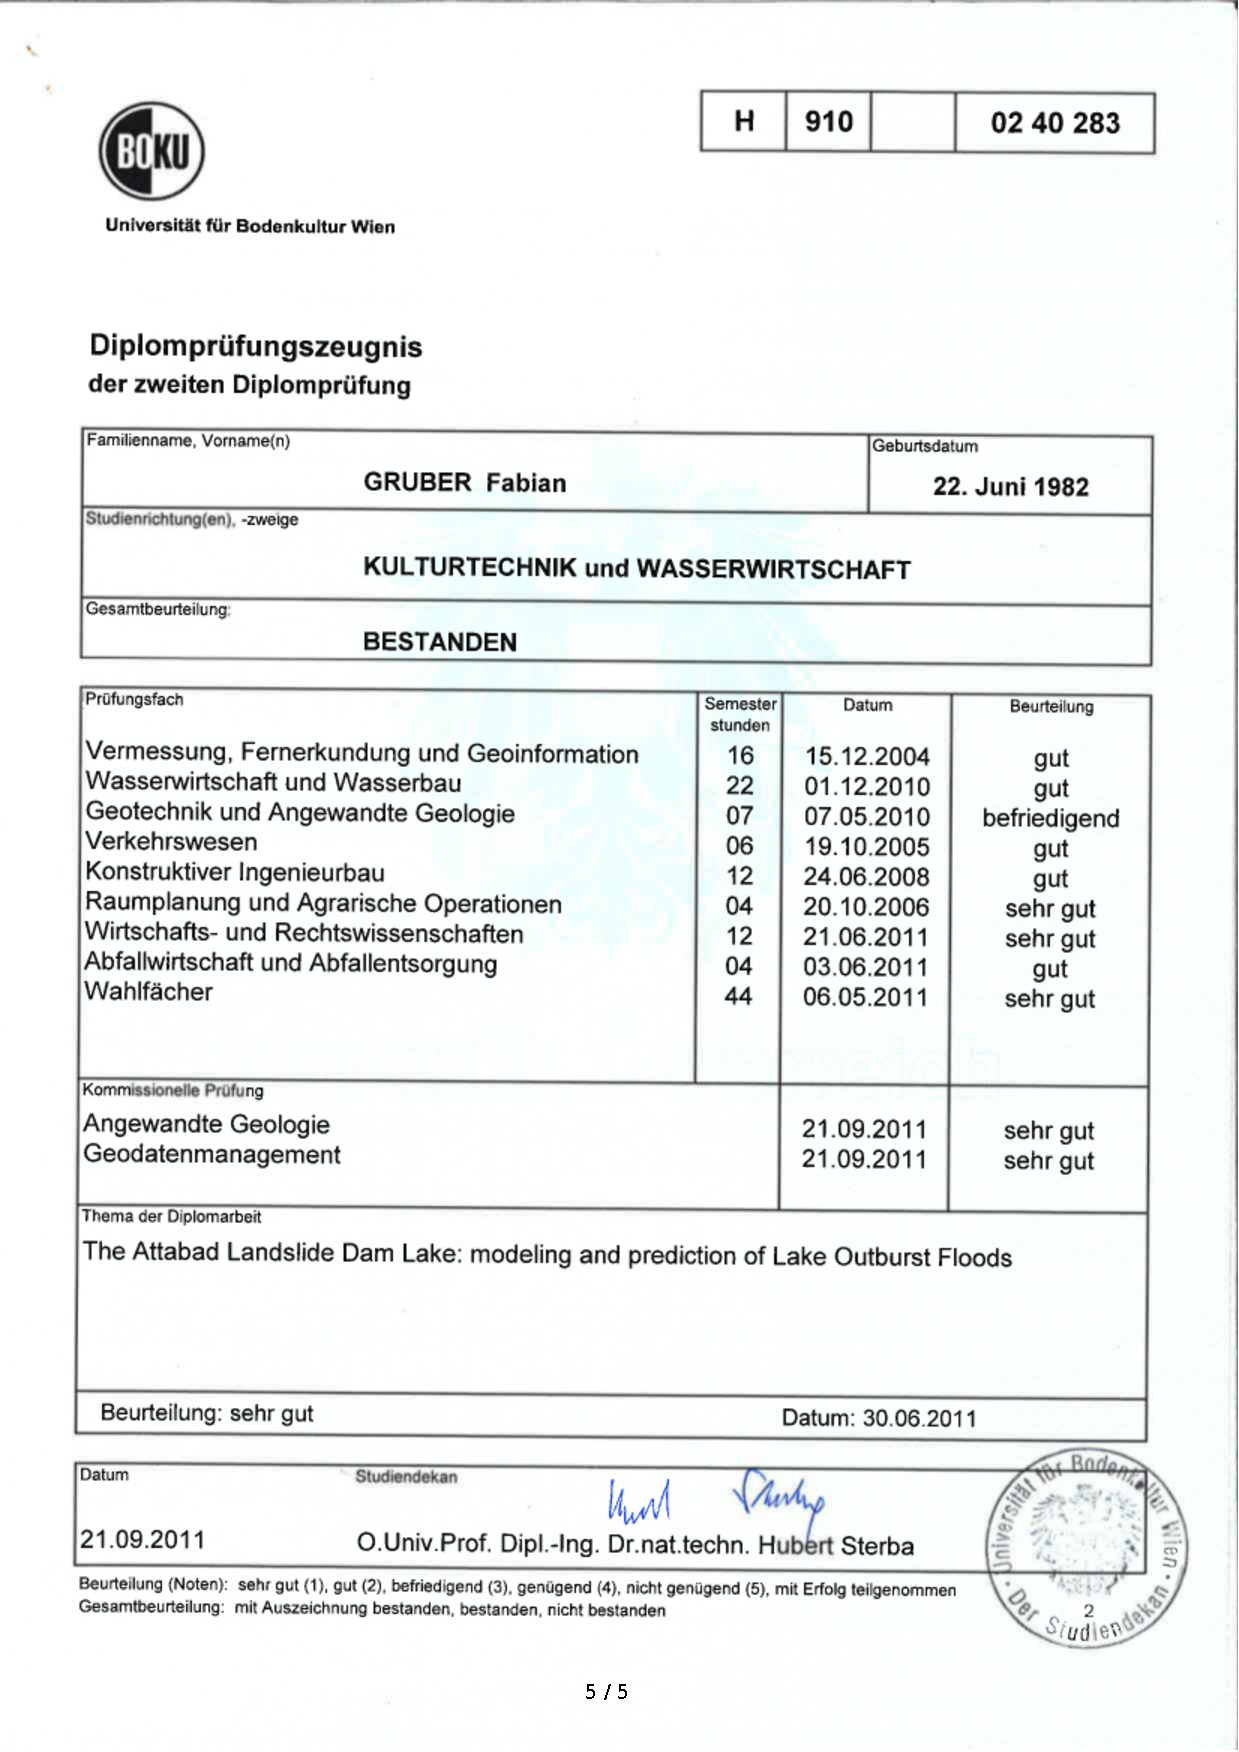
\includepdf{DP1_5von5.pdf}
%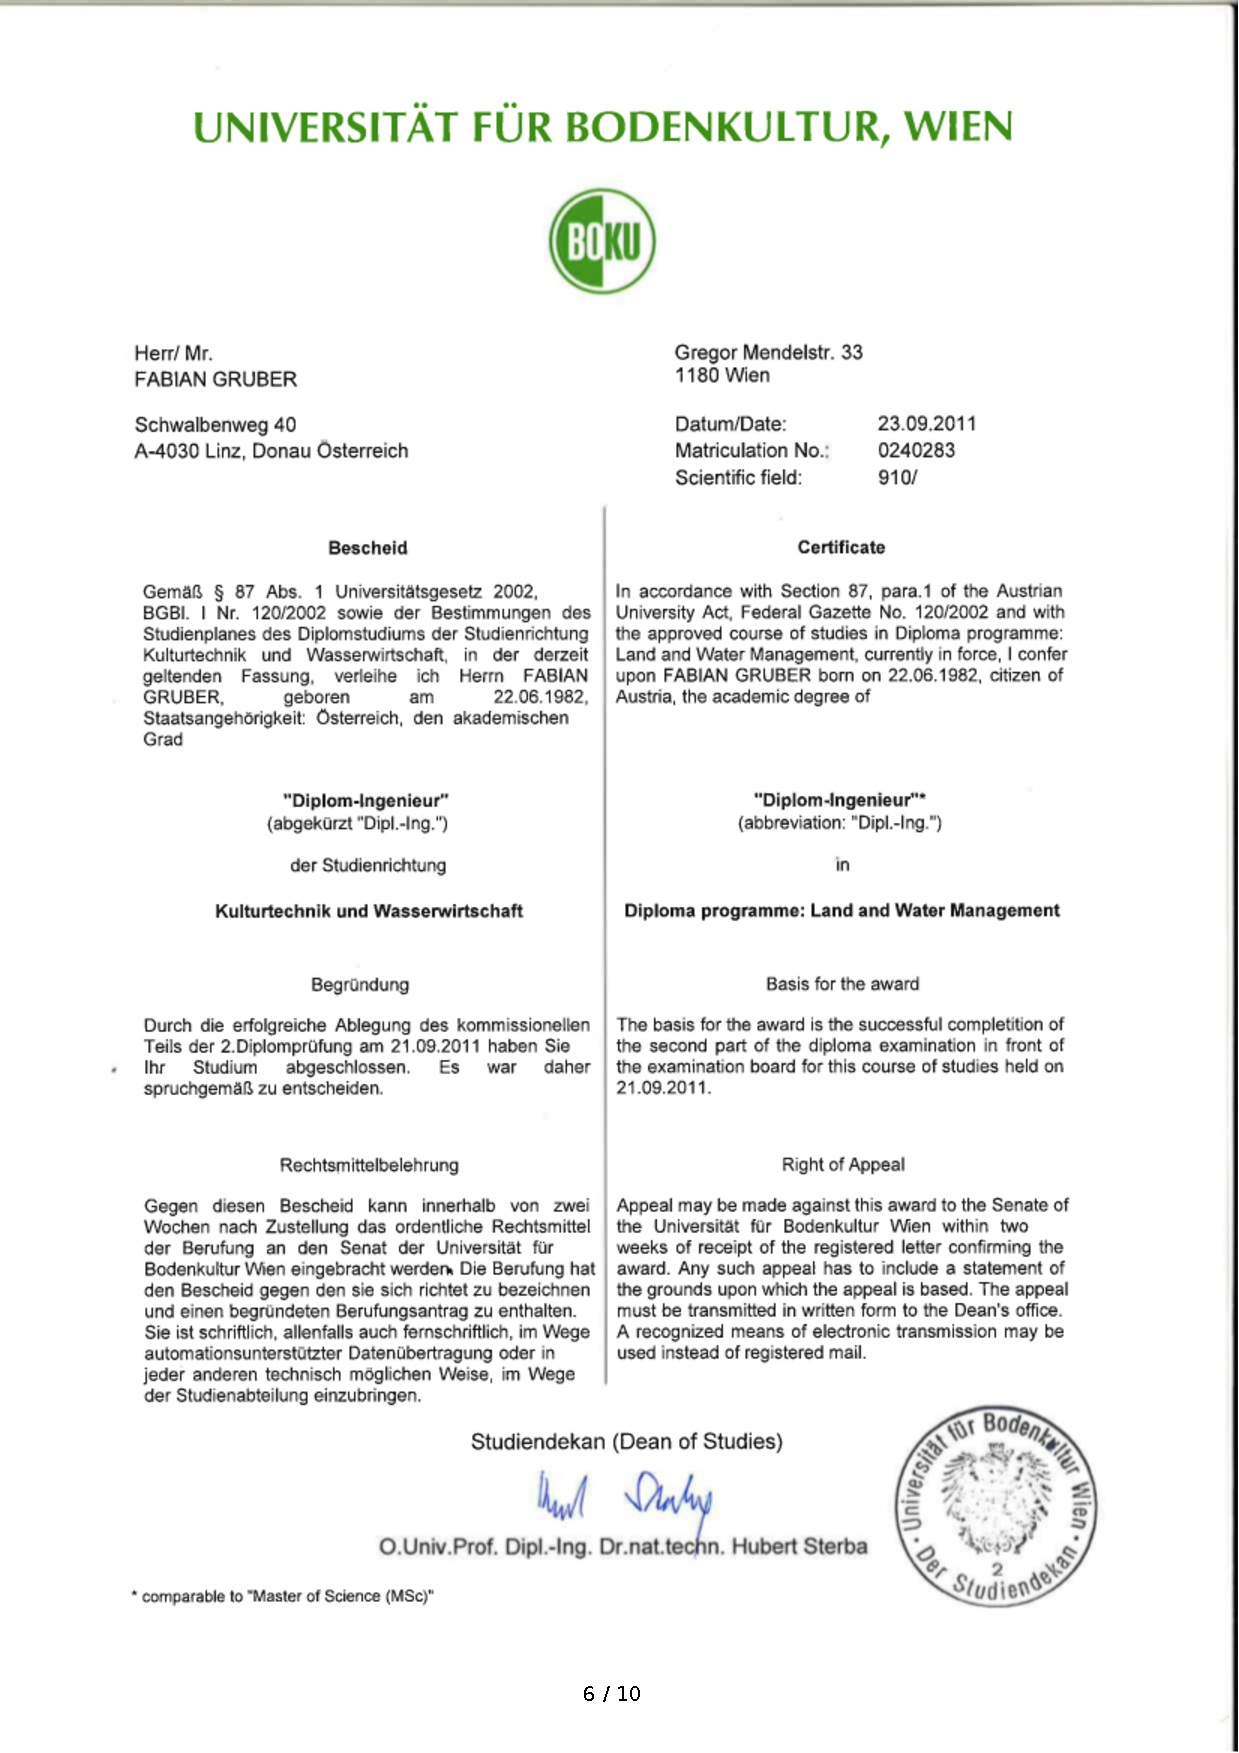
\includepdf{DP_6.pdf}
%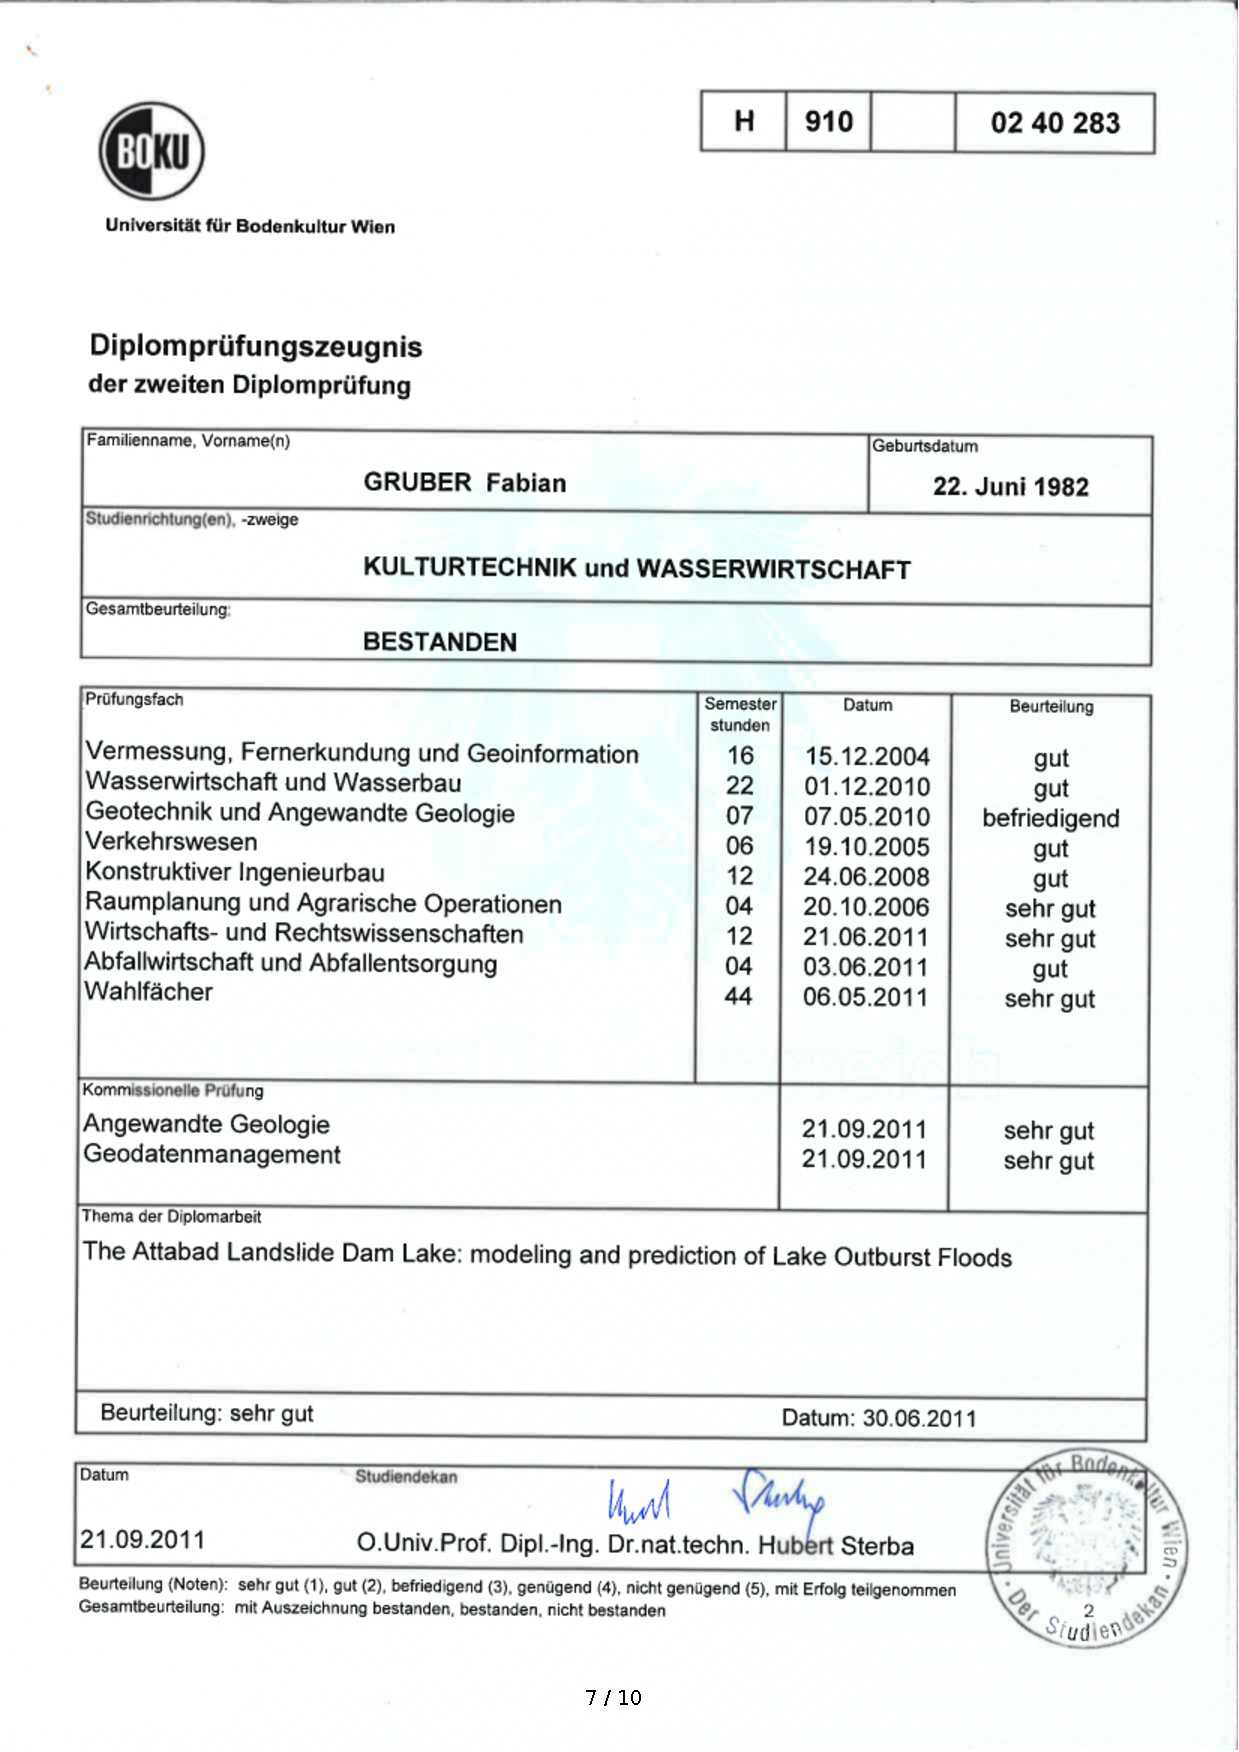
\includepdf{DP1_7.pdf}
%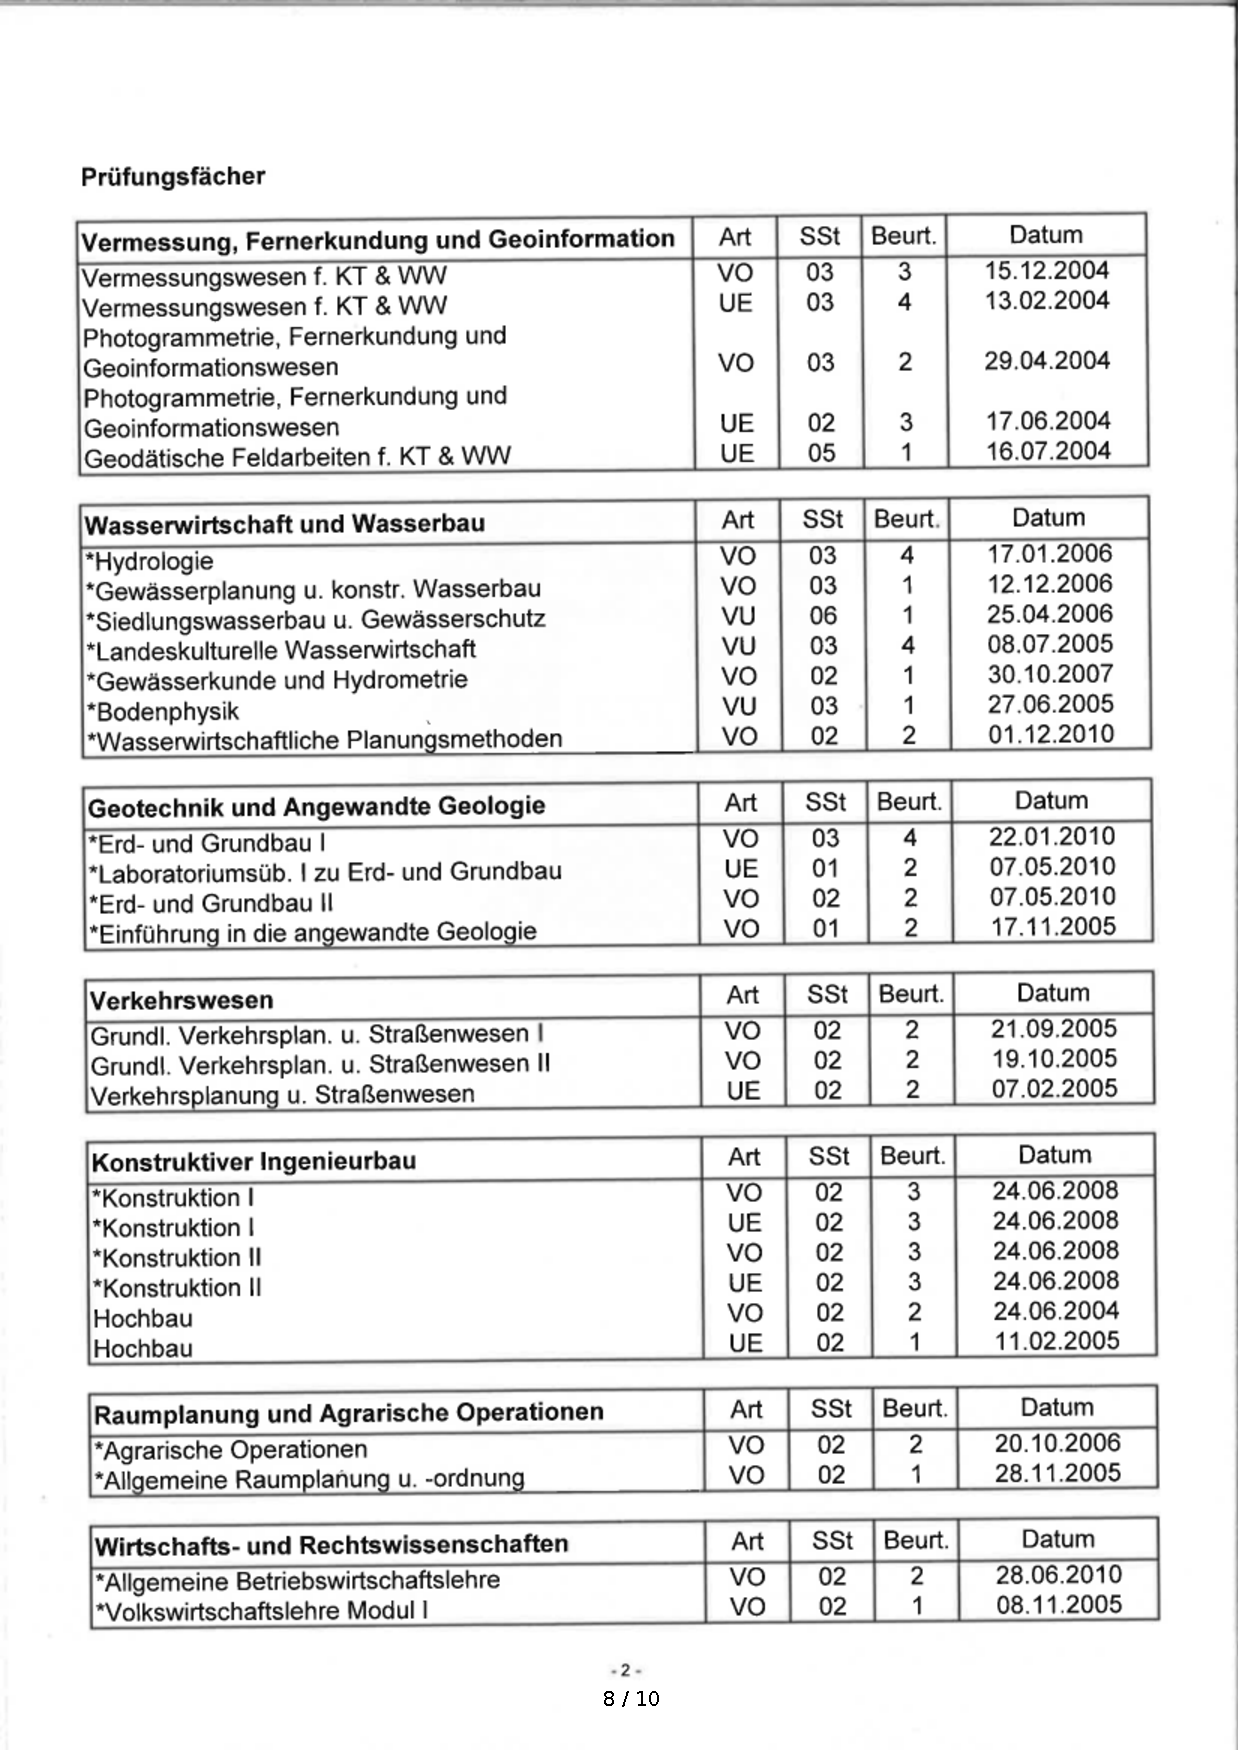
\includepdf{DP2_8.pdf}
%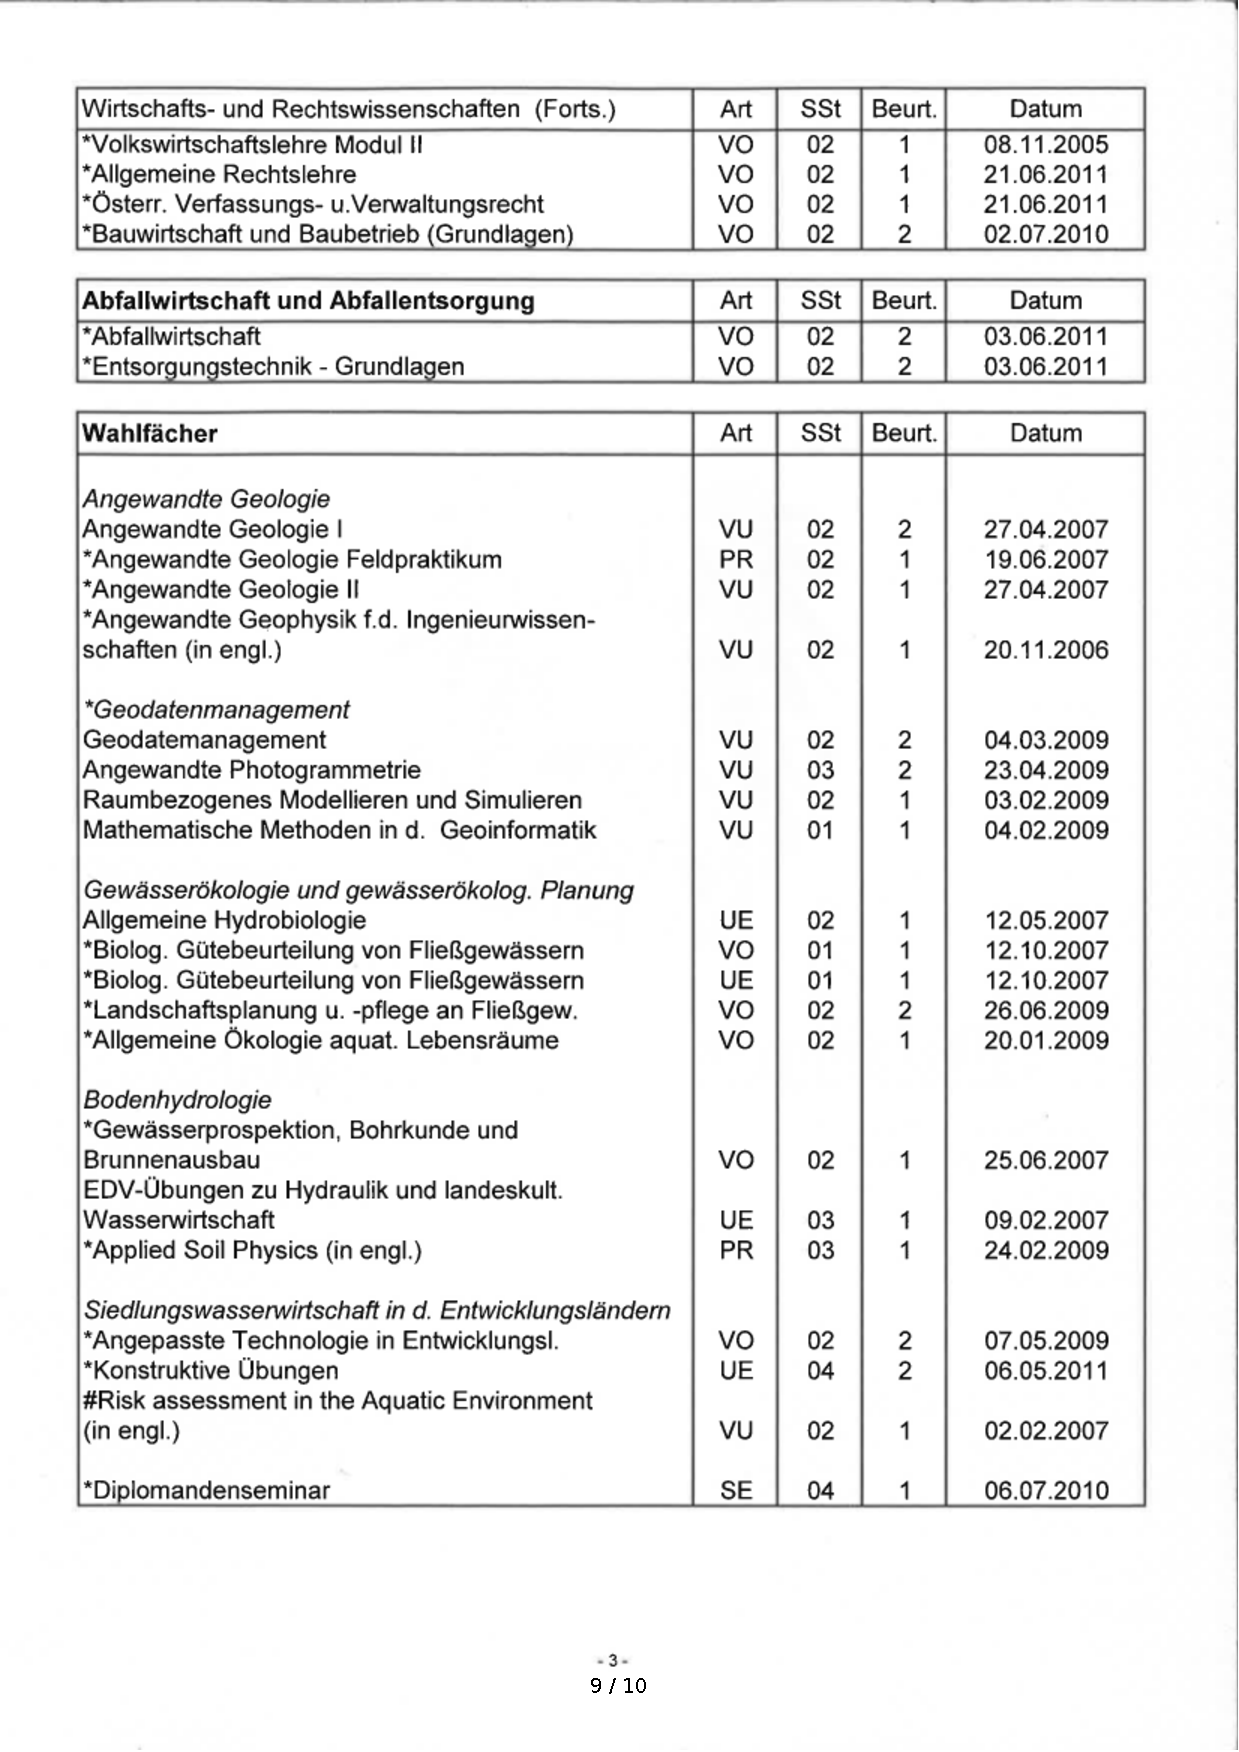
\includepdf{DP3_9.pdf}
%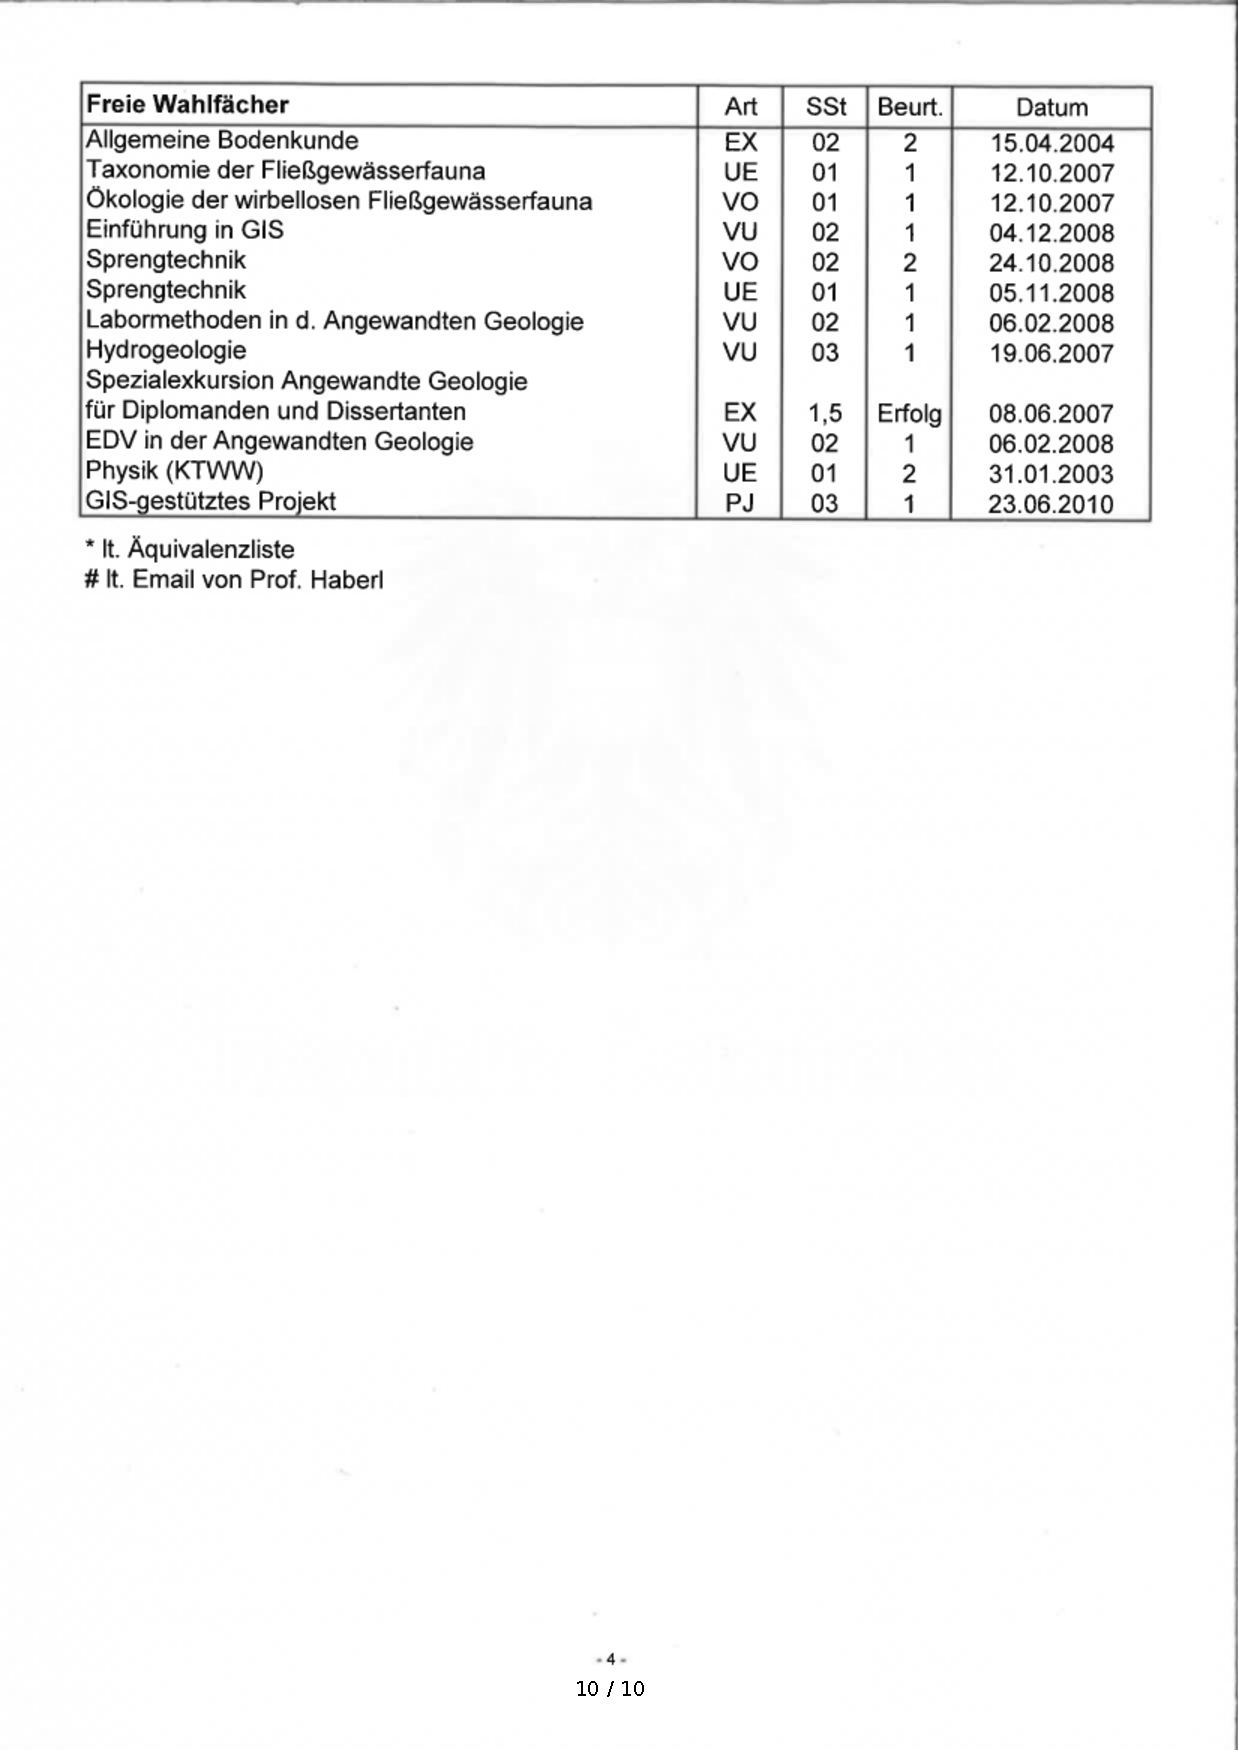
\includepdf{DP4_10.pdf}
\end{document}


%% end of file `template.tex'.
